\section{Results}
\label{results}

At the time of this publication the ontology has an open git
repository\footnote{Note for the editors: The publishing of the repository is
being subject to export control, we would update the links accordingly in the
camera-ready version. }. This repository has developer documentation where the
motivating scenarios along with their competency questions are written. A quick
introduction for developers is also part of this documentation. This
documentation is written using exclusively markdown files which can be rendered
into webpages with different packages, we opt for using
MkDocs\footnote{https://www.mkdocs.org/} because of its simplicity. For the
ontology documentation and the IRI resolution, we are still exploring solutions.
We are tending towards Widoco\footnote{https://github.com/dgarijo/Widoco}.

We implemented a Python test suite that allows the incremental development of
the ontology using competency questions. This suite classifies the queries into
two types. Those who act on classes (TBox) like \hyperref[CQ1.1]{CQ 1.1} and
those that act on individuals (ABox) like \hyperref[CQ2.0]{CQ 2.0}. To handle
the ABox queries we rewrite the natural language questions as ASK queries in
SPARQL  that returns either true or false values. We also declare a model in
Turtle Syntax that instantiates the referred classes. For example
\hyperref[CQ2.0]{CQ 2.0} is written as listing \ref{lst:1} and its corresponding
model \ref{lst:2} populates the ABox. The TBox questions are evaluated by
checking entailment using DL queries such as the one in listing \ref{lst:3}
which corresponds to \hyperref[CQ1.1]{CQ 1.1}.

\begin{listing}[h]
    
    \begin{minted}[fontsize=\small]{sparql}
        ASK WHERE {
            SELECT (COUNT(?parkingSpaces) AS ?vehicleCapacity)  
            WHERE  {  :SomeParkingArea obo:BFO_0000178 ?parkingSpaces . 
                      ?parkingSpaces rdf:type obo:CHIO_00000002 . }
            HAVING ( ?vehicleCapacity = 2 ) }
    \end{minted}
    \caption{Example ABox query. (Given a parking area with two parking places) What is the (vehicle) capacity of parking lot P? (2). The namespaces are omitted.}
    \label{lst:1}
\end{listing}

\begin{listing}[h]
    \begin{minted}[fontsize=\small]{turtle}
        :SomeParkingSpaceA a chio:CHIO_00000002 .
        :SomeParkingSpaceB a chio:CHIO_00000002 .
        :SomeParkingArea a chio:CHIO_00000001 ;
                         obo:BFO_0000178 :SomeParkingSpaceA,
                                         :SomeParkingSpaceB .
    \end{minted}
    \caption{Example ABox instances. Two charging spaces (that can hold at most one car at a time) are part of some parking area. Namespace prefixes are omitted, the chio namespace refers to the charging ontology.}
    \label{lst:2}
\end{listing}

\begin{listing}[h]
    \begin{minted}[fontsize=\small]{text}
        'charging station' SubClassOf 'parking facility' 
            and 'has continuant part' some 'charging column'
    \end{minted}
    \caption{Example DL Query used to evaluate TBox competency. A charging station is a kind of parking facility and has charging columns as parts.}
    \label{lst:3}
\end{listing}

Since we aim for a high rate of reusability, most of the efforts have been aimed
towards finding concepts from existing ontologies. We import the entire CCO
version of the BFO which already includes basic RO axioms. We import the
excerpts from OEO and CCO mentioned in section \ref{methodology}, we do this by
providing scripts that ensure transparency and reproducibility. These scripts
point to specific versions of the ontologies that can be updated based on
developing needs. In some cases, we reimplemented terms and pointed out the ones
from other ontologies by using mappings. This was the case for the axioms from
the TPSO Parking Ontology (figure \ref{parkingfig}). Our interpretation of
parking areas and spaces is similar, but we rely on the mereology of BFO.
Instead of assigning the charging stations to parking spaces directly we opt to
use the facility axioms from CCO. These implementations can be visualized in
figure \ref{parkingchio}.

\begin{figure}[h]
    \centering
    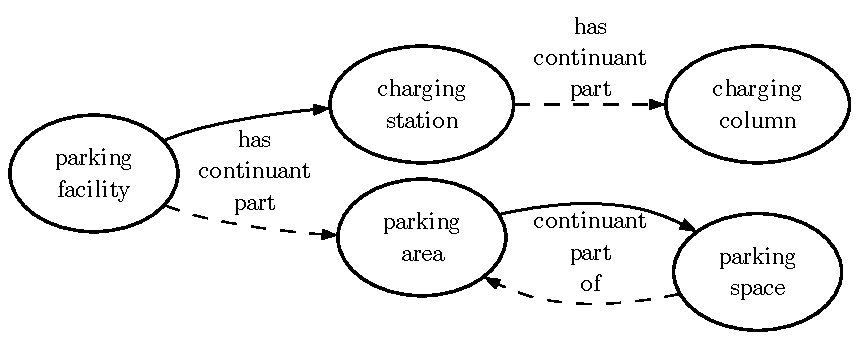
\includegraphics{images/CHIOParking.pdf}
    \caption{Parking area, place, and facility implementations in our ontology. This model builds on the taxonomy of the CCO Facility Ontology. Solid arrows represent super-class relations.}
    \label{parkingchio}
\end{figure}



    